\section*{Motivation}
Betrachte die Temperatur in einem Raum, modelliert durch $\Omega = (0,1)^2$.
Die Temperatur in jedem Punkt im Raum kann als Funktion $u \colon \Omega \to \R $ aufgefasst werden.
Gegeben sei außerdem eine Wärmequelle, modelliert als $f \colon \Omega \to \R $  im Raum und eine Temperatur der Wände von $u(x)=0, x \in \partial \Omega = (\{0,1\} \times [0,1] ) \cup ([0,1] \times \{0,1\} $.
Nach einer gewissen (unendlichen) Zeit wird die Temperatur ein Gleichgewicht annehmen, welches die Lösung einer \emph{partiellen Differentialgleichung}
\begin{equation}
	\label{eqn:löser}
\begin{cases}
	-\Delta u(x) = f(x) & x \in \Omega \\
	u(x) = 0 & x \in \partial \Omega
\end{cases}
\end{equation}
geschrieben werden.
\begin{definition}
Der Laplace-Operator $\Delta$ ist definiert als: 
\[
\Delta u(x) = \frac{\partial^2 u}{\partial x_1^2}(x_1,x_2) + \frac{\partial^2 u}{\partial x_2^2}(x_1,x_2 , x = \begin{bmatrix}
x_1 \\ x_{2} 
\end{bmatrix} \in \Omega
\]
falls $u$ genügend oft differenzierbar ist.
\end{definition}
Das Ziel ist es, $u$ zuberechnen, wenn $f$ gegeben ist. Das Problem im Allgemeinen ist, dass \eqref{eqn:löser} nicht von Hand lösbar ist, daher erfolgt die Lösung mit Hilfe des Computers. Dies ist generell nur approximativ möglich.
\paragraph{Beobachte:} Für eine genügend oft differenzierbare Funktion $g \colon \R \to \R $, gilt 
\[
g'(x)= \lim_{h \to 0} \frac{g(x+h)-g(x)}{h} \approx \frac{g(x)-g(x-h)}{h} \approx \frac{g(x+h)-g(x)}{h}
\]
für ein kleines h. Also:
\begin{align*}
	g"(x) &\approx \frac{g'(x+h)-g'(x)}{h} \\
	      &\approx \frac{\frac{g(x+h)-g(x)}{h}-\frac{g(x)-g(x-h)}{h}}{h} \\
	      &\approx \frac{g(x+h)-2g(x)+g(x-h)}{h^2}
\end{align*}
Unsere Idee ist nun, die zweiten Ableitungen im Laplace-Operator durch diese Aproxximationen zu erstezen:
\begin{align*}
\frac{\partial^2 u}{\partial x_{1}^2}(x_1,x_2) \approx \frac{u(x_1+h,x_2) - 2u(x_1,x_2) + u(x_1-h,x_2)}{h^2} \\
\frac{\partial^2 u}{\partial x_{2}^2}(x_1,x_2) \approx \frac{u(x_1,x_2+h) - 2u(x_1,x_2) + u(x_1,x_2-h)}{h^2}
\end{align*}
Für eine systematische Approximation der Ableitungen führen wir ein Gitter ein. Wähle $n \in \N$ und eine Schrittweite $h=\frac{1}{n}$.

%missing picture

Wir betrachten $u$ nur noch an den Gitterpunkten $x_{i,j}$ und suchen Approximationen $u_{i,j} \approx u(x_{i,j})$ . Wir erhalten:
\begin{equation}
	\label{eqn:komplex}
\begin{rcases}
	\frac{1}{h^2}(4u_{i,j} - u_{i-1,j} -u_{i+1,j} -u_{i,j-1} - u_{i,j+1} = f_{i,j} = f(x_{i,j}) , x_{i,j} \in \Omega \\
	u_{i,j} = 0  , x_{i,j} \in \partial \Omega \text{, also } i,j \in \{0,n\}  
\end{rcases}
\end{equation}
Wir erhalten also ein lineares Gleichungssystem $An=f$ mit $N=(n-1)^2$ Unbekannten. Gemäß \eqref{eqn:komplex} hat $A$ nur fünf Einträge pro Zeile bzw. Spalte, insgesamt also $\mathcal{O}(N)$ Einträge. 
$A$ ist demnach extrem dünn besetzt.
\begin{example}
	\label{eg:löser1}
Sei $n=4$. Dann ist $h=\frac{1}{4}$ und 

%nette grafik muss noch kommmen
\end{example}
\paragraph{Beobachtung:} Wir haben das Lösen einer partiellen Differentialgleichung auf das Lösen eines linearen Gleichungssystem reduziert. Jedoch ist für die Lösung $u$ von \eqref{eqn:löser} zu erhalten, oft $1 \ll n$ nötig. Die  Größe des linearen Gleichungssystem ist $\mathcal{O}(n^2) = \mathcal{O}(N)$. Das Lösen des linearen Gleichungssystem ist demnach $\mathcal{O}(N^3)$, was in der Realität praktisch nicht durchführbar ist. Dies liegt daran, dass die $LR$-Zerlegung von $A$ im ALlgemeinem viel mehr nicht-null Einträge hat als $A$.\\
Um die Dünnbestztheit von $A$ besser auszunutzen, sodass die Faktoren der (modifizierten LR-Zerlegung ebenfalls dünnbestetzt sind betrachten wir die Systemmatrix $A$ als ADjazentmatrix eines Graphen $G_A$.
\begin{example}
Der Graph $G_A$ zur Matrix aus Beispiel \ref{eg:löser1} ist:
\begin{center}
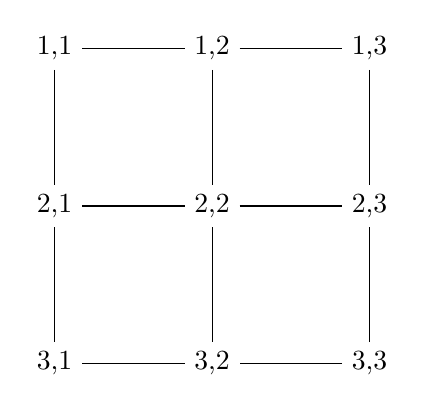
\begin{tikzpicture}[node distance = 2cm, auto]
\node (1) {1,1};
\node (2) [right of=1] {1,2};
\node (3) [right of=2] {1,3};
\node (4) [below of=1] {2,1};
\node (5) [below of=2] {2,2};
\node (6) [below of=3] {2,3};
\node (7) [below of=4] {3,1};
\node (8) [below of=5] {3,2};
\node (9) [below of=6] {3,3};

\path [-] (1) edge node {} (2);
\path [-] (1) edge node {} (4);
\path [-] (2) edge node {} (5);
\path [-] (2) edge node {} (3);
\path [-] (3) edge node {} (6);
\path [-] (9) edge node {} (8);
\path [-] (5) edge node {} (8);
\path [-] (5) edge node {} (4);
\path [-] (4) edge node {} (7);
\path [-] (9) edge node {} (6);
\path [-] (5) edge node {} (6);
\path [-] (7) edge node {} (8);











\end{tikzpicture}
\end{center}
\end{example}
